\chapter{Cronograma}
\label{ch:Crono}

En la Tabla  \ref{tabla:tareas} se muestra las actividades a desarrollar durante la investigación y elaboración del proyecto. La Figura 6.1 muestra el diagrama de Gantt correspondiente a las actividades.

\begin{table}[h]
\centering
\begin{tabular}{||c|l||}
\hline
\textbf{Tarea \#} & \textbf{Tarea a realizar} \\[1.5ex]
\hline\hline
1 & Investigación sobre las arquitecturas de lógica reconfigurable\\[1.5ex]
\hline
2 & Configuración del entorno de desarrollo y herramientas \\[1.5ex]
\hline
3 & Revisión y ajuste de los módulos en código RTL \\[1.5ex]
\hline
4 & Ejecución de los primeros procesos de síntesis lógica \\[1.5ex]
\hline
5 & Generación del archivo de configuración \\[1.5ex]
\hline
6 & Descripción de hardware de los dos circuitos de prueba \\[1.5ex]
\hline
7 & Procesamiento del filtro digital y el multiplicador de enteros \\[1.5ex]
\hline
8 & Extracción de las métricas finales \\[1.5ex]
\hline
9 & Análisis crítico de los puntos de trade-off  \\[1.5ex]
\hline
10 & Elaboración del informe escrito \\[1.5ex]
\hline
11 & Entrega del informe final \\[1.5ex]
\hline
12 & Defensa del proyecto \\[1.5ex]
\hline
\end{tabular}
\caption{Lista de tareas del proyecto}
\label{tabla:tareas}
\end{table}

\newpage

En la siguiente figura \ref{Gannt}, presentamos un Diagrama de Gantt que muestra gráficamente el cronograma de nuestro proyecto. Este diagrama nos permite visualizar con claridad la planificación de las diferentes actividades y su duración a lo largo de las semanas. Las tareas de cada objetivo específico están representadas por barras horizontales, cuya longitud es proporcional a la duración estimada de cada tarea. La organización de estas barras a lo largo de la línea temporal proporciona una perspectiva clara de cuándo y cómo se llevarán a cabo las actividades, facilitando así la gestión del tiempo y la distribución de los recursos. Las superposiciones indican la simultaneidad de tareas y las intersecciones demuestran los puntos donde las actividades están interconectadas. Este diagrama es la hoja de ruta visual de nuestro proyecto, y nos ayudará a mantenernos en la senda correcta, asegurando que todas las tareas se completen en los plazos establecidos.


         \begin{figure}[H]
		  \centering 
			  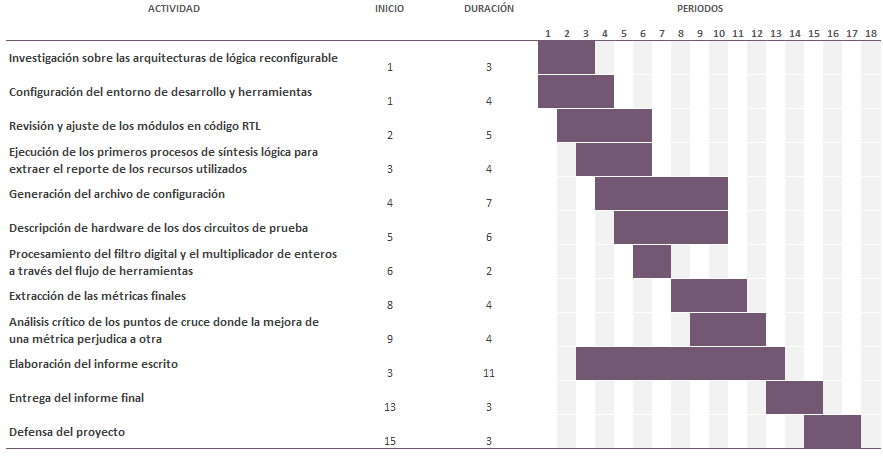
\includegraphics[scale=0.7]{pics/Cronograma.png}
			  \caption{Diagrama de Gantt de las actividades a realizar}
    		  \label{Gannt}
		\end{figure}
